\documentclass[a4paper]{article}
\usepackage[margin=1in]{geometry}
\usepackage{graphicx}
\usepackage{hyperref}
\usepackage{amsmath}
\usepackage{booktabs}
\usepackage{subcaption}
\usepackage{tikz}
\usepackage{pgfplots}
\usepackage{float}

\title{\textbf{VE216 Lab 2 Report\\AM Radio}}
\author{
    \Large Han Yibei
    \normalsize 519370910123
}
\date{\today}

\begin{document}
    \maketitle
    \tableofcontents
    \newpage




    \section{Objectives}
    \begin{itemize}
        \item Understand the principle of envelope detector and its relationship with Amplitude Demodulation.
        \item Review op amp circuits.
    \end{itemize}

    \section{Theoretical background}
    \subsection{Transimitted Signal}
    The transmitted AM signal follows form $x(t) = (A+bs(t))cos(\omega_ct+\theta))$, where $cos(\omega_ct+\theta))$ is the carrier. The presense of $A$ and $b$ is important for envelope detection. The efficiency of signal transmitting can be calculated by the following equation
    \begin{equation*}
        \frac{max(bs(t))-min(bs(t))}{2A} \times 100 \%
    \end{equation*}

    \subsection{Pre-built Front-end: Antenna \& Tuned RLC circuit}
    The front-end consists of a tunned RLC circuit, a field effect transistor pre-amplifier and a mixer. The RLC circuit can be modeled by the circuit shown below \autoref{fig:LC_diagram}.
    \begin{figure}[h]
        \centering
        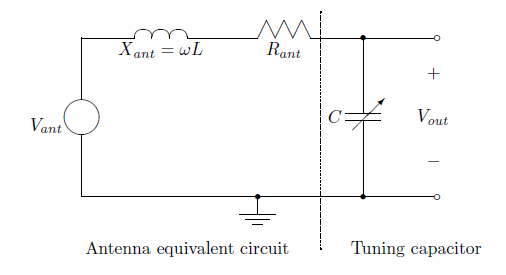
\includegraphics[width=10cm]{tuned.png}
        \caption{Tuned RLC Circuit diagram}
        \label{fig:LC_diagram}
    \end{figure}
    It is easy to verify that the circuit serves as a bandpass filters
    \begin{equation*}
        H(jw) = \frac{\frac{1}{c\omega j}}{\frac{1}{c\omega j}+L\omega j+R} = \frac{1}{LC(j\omega)^2+RC(j\omega)+1}
    \end{equation*}
    where the capacitor is controlled by the radio listener.
    
    \subsection{RLC Resonant Circuit}
    When the current in the circuit is maximized, the circuit is under the situation of resonant. The resonant frequency can be calculated by the following equation
    \begin{equation*}
        f_{res} = \frac{1}{2\pi} \frac{1}{\sqrt{LC}}Hz
    \end{equation*}
    The 3dB bandwidth
    \begin{equation*}
        BW_{3dB} = \frac{1}{2\pi} \frac{R}{L}Hz
    \end{equation*}
    The quality factor is
    \begin{equation*}
        Q = 2\pi f_{res} \frac{L}{R}
    \end{equation*}

    \subsection{Amplifier \& Mixer in the Front-end}
    To demodulate the signal, we need to first move the signal to the frequency range where the IF filter works with the mixer. For example, an AM signal has been modulated (shifted) from the baseband
    \begin{equation*}
        x(t) = (A+bs(t))cos(\omega_ct+\phi)
    \end{equation*}
    the output of mixer is 
    \begin{equation*}
        x(t) = (A+bs(t))cos(\omega_ct+\phi)cos(\omega_{LO}t+\theta)
    \end{equation*}
    We already know that cosine modulation in the time domain means moving in the frequency domain, so the way amplifiers and mixers work can be defined as \autoref{fig:LO}.
    \begin{figure}[h]
        \centering
        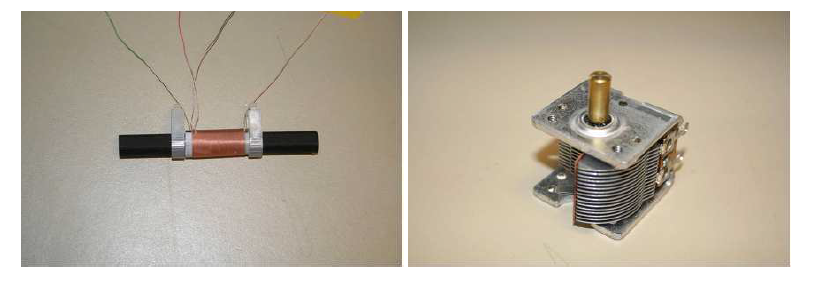
\includegraphics[width=0.8\textwidth, trim={0 0 0 0cm}, clip]{loop.png}
        \caption{(a) original signal, (b) modulated signal, (c) signal after mixer}
        \label{fig:LO}
    \end{figure}

    \subsection{IF Filter}
    We know that mixers can be used to move the frequency of an AM signal to the desired range. This is especially important for filtering when the filter range is fixed like the IF filter. Usually, we have two choice of $f_{LO}$
    \begin{equation*}
        f_{LO} = f_c - f_{IF}
    \end{equation*}
    or 
    \begin{equation*}
        f_{LO} = f_c + f_{IF}
    \end{equation*}
    When $x(t)$ isn't the only signal in the channel. Usually, other signals of different frequencies will also enter this range, interfering with the final demodulation $x(t)$. The situation is shown in \autoref{fig:IF_1} \& \autoref{fig:IF_2}
    \begin{figure}[h]
        \centering
        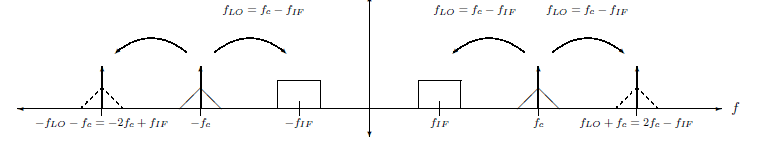
\includegraphics[width=0.8\textwidth, trim={0 0 0 0cm}, clip]{band1.png}
        \caption{when $f_{LO} = f_c - f_{IF}$}
        \label{fig:IF_1}
    \end{figure}
    \begin{figure}[h]
        \centering
        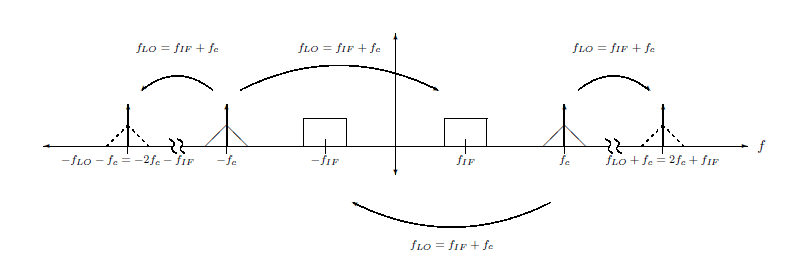
\includegraphics[width=0.8\textwidth, trim={0 0 0 0cm}, clip]{band2.png}
        \caption{when $f_{LO} = f_c + f_{IF}$}
        \label{fig:IF_2}
    \end{figure}

    So, before we mix the signals, we should add a band-pass tunable signal to the AM signal that is wider than the IF signal, but narrow enough to filter out those potentially interfering signals.

    \subsection{A simple Butterworth Filter Realization of the IF Filter}
    In the lab, we will construct an op amp-based IF filter, which is not optimal, but is easy to obtain.

    It is shown in prelab that the frequency response is 
    \begin{equation*}
        H_{IF}(s) = \frac{a_1s}{a_2s^2+a_3s+a_4}
    \end{equation*}
    where
    \begin{align*}
        a_1 & = -R_2R_3C/(R_1+R_2) \\
        a_2 & = R_1R_2R_3C^2/(R_1+R_2) \\
        a_3 & = 2R_1R_2C/(R_1+R_2) \\
        a_4 & = 1 \\ 
    \end{align*}
    and through educated approximation, we can easily verify that 
    \begin{align*}
        & f_{res} = \frac{1}{2\pi} \sqrt{\frac{R_1+R_2}{R_1R_2R_3C^2}} \\
        & H_{max} = R_3/R_1 \\
        & BW  = 1/R_3C\pi \\
    \end{align*}

    \section{Experiment Procedures}
    \subsection{Modulated Sine Wave}
    \begin{itemize}
        \item Set the load of the function generator to be 50 Ohm
        \item Use the function generator to generate a modulated sine wave withe baseband frequency 1kHz and modulating frequency 100kHz.
        
        The original signal should have 4V Vpp.

        The carrier signal should be sine wave as well.

        The modulation index should be 0.5
        \item Directly connect the generator to the oscilloscope to verify the generated waveform. Store the images with time division $200\mu s$ and $20\mu s$
    \end{itemize}

    \subsection{Modulated Triangular Wave}
    \begin{itemize}
        \item Repeat Part 1, with the only different that the original signal should have triangular shape.
    \end{itemize}


    \subsection{Envelop Detector}
    \begin{itemize}
        \item Assemble the circuit using $R=75k\Omega$ and $C=2.2nF$
        \item Use the envelope detector to "demodulate" the two signals in Part 1 and 2. Store images at $200\mu s$ and $20\mu s$ and be sure to display both CH1 and CH2
    \end{itemize}
    \subsection{Amplifier}
    \begin{itemize}
        \item Use the function generator to generate a 5kHz sine wave with 500 mV Vpp
        \item Assemble the circuit using $R_1 = 15k\Omega$, $R_2 = 5.6k\Omega$, $R_3 = 82k\Omega$ and $C = 220\mu F$
    \end{itemize}

    \section{Experimental Results}
    \subsection{Modulated Sine Wave}
    The original sine wave is $s(t)=2cos(\omega t+\theta)$. With index=0.5, the amplitude is 4Vpp. And the carrier should be 
    $$y(t)=(2cos(\omega t+\theta)+4)cos(\omega_ct+\theta_c)$$
    where $\omega=1kHz/2\pi$ and $\omega_c=100kHz/2\pi$\\

    The generated wave is shown as the yellow part
    \begin{figure}[H]
        \centering
        \begin{subfigure}{0.4\textwidth}
            \includegraphics[width=\textwidth, trim={0 0.3cm 2cm 0.6cm}, clip]{sine1.jpg}
            \caption{Time Division $20\mu s$}
        \end{subfigure}
        \begin{subfigure}{0.4\textwidth}
            \includegraphics[width=\textwidth, trim={0 0.3cm 2cm 0.6cm}, clip]{sine2.jpg}
            \caption{Time Division $200\mu s$}
        \end{subfigure}
        \caption{Modulated Sine Wave}
    \end{figure} 

    \subsection{Modulated Triangular Wave}
    The original triangular wave is 
    $$s(t)=2\sum_{n=-\infty}^\infty tri(4ft-1+4n)-tri(4ft+1+4n)$$
    With index=0.5, the amplitude is 4Vpp. And the carrier should be 
    $$y(t)=(2\sum_{n=-\infty}^\infty tri(4ft-1+4n)-tri(4ft+1+4n)+4)cos(\omega_ct+\theta_c)$$
    where $f=1kHz$ and $\omega_c=100kHz/2\pi$\\
    The waveform is shown in picture(yellow part)
    The generated wave is shown as the yellow part
    \begin{figure}[H]
        \centering
        \begin{subfigure}{0.4\textwidth}
            \includegraphics[width=\textwidth, trim={0 0.3cm 2cm 0.6cm}, clip]{tri1.jpg}
            \caption{Time Division $20\mu s$}
        \end{subfigure}
        \begin{subfigure}{0.4\textwidth}
            \includegraphics[width=\textwidth, trim={0 0.3cm 2cm 0.6cm}, clip]{tri2.jpg}
            \caption{Time Division $200\mu s$}
        \end{subfigure}
        \caption{Modulated Triangular Wave}
    \end{figure} 

    \subsection{Envelope Detector}
    \paragraph{Sine wave}
    Shown in the figure:
    \begin{figure}[H]
        \centering
        \begin{subfigure}{0.4\textwidth}
            \includegraphics[width=\textwidth, trim={0 0.3cm 2cm 0.6cm}, clip]{sine1.jpg}
            \caption{Time Division $20\mu s$}
        \end{subfigure}
        \begin{subfigure}{0.4\textwidth}
            \includegraphics[width=\textwidth, trim={0 0.3cm 2cm 0.6cm}, clip]{sine2.jpg}
            \caption{Time Division $200\mu s$}
        \end{subfigure}
        \caption{Modulated Sine Wave with envelope}
        \label{fig:sin1}
    \end{figure} 

    \paragraph{Triangular Wave} 
    Shown in the figure
    \begin{figure}[H]
        \centering
        \begin{subfigure}{0.4\textwidth}
            \includegraphics[width=\textwidth, trim={0 0.3cm 2cm 0.6cm}, clip]{tri1.jpg}
            \caption{Time Division $20\mu s$}
        \end{subfigure}
        \begin{subfigure}{0.4\textwidth}
            \includegraphics[width=\textwidth, trim={0 0.3cm 2cm 0.6cm}, clip]{tri2.jpg}
            \caption{Time Division $200\mu s$}
        \end{subfigure}
        \caption{Modulated Triangular Wave with envelope}
    \end{figure} 

    \subsection{Amplifier}
    The measured input and output are shown in the figure\\
    \begin{figure}[H]
        \centering
        \includegraphics[width=8cm]{amp.jpg}
        \caption{Input and Output with amplifier}
    \end{figure}
    Experimentally, we get the output $\frac{V_o}{V_i}=\frac{960mV}{250mV}=3.84$\\
    Theoretically, we get that $$\frac{V_o}{V_i}=|\frac{(R_1+R_2)c\omega j}{R_2(c\omega j+\frac{1}{R_3})}|=3.68$$\\
    Experimental outcome fit the theoretical outcome.


    \section{Conclusion}
    In this lab we 
    \begin{itemize}
        \item Learn about resonance phenomena and simple RLC bandpass filters.
        \item Learn about the mechanism of antennas
        \item Learn basic superheterodyne receiver operating principles
        \item Construct a operational superheterodyne
    \end{itemize}
    And the error may cause by the resist of wire. Also, there may exist simulation error of the appliance. In the amplifier part, the error may caused by the unstable cursor.

\end{document}